% $Header: /cvsroot/latex-beamer/latex-beamer/solutions/conference-talks/conference-ornate-20min.en.tex,v 1.6 2004/10/07 20:53:08 tantau Exp $

\documentclass{beamer}

% This file is a solution template for:

% - Talk at a conference/colloquium.
% - Talk length is about 20min.
% - Style is ornate.



% Copyright 2004 by Till Tantau <tantau@users.sourceforge.net>.
%
% In principle, this file can be redistributed and/or modified under
% the terms of the GNU Public License, version 2.
%
% However, this file is supposed to be a template to be modified
% for your own needs. For this reason, if you use this file as a
% template and not specifically distribute it as part of a another
% package/program, I grant the extra permission to freely copy and
% modify this file as you see fit and even to delete this copyright
% notice.


\mode<presentation>
{
%  \usetheme{Warsaw}
%  \usetheme{Boadilla}
%  \usetheme{Goettingen}
%  \usetheme{Hannover}
%  \usetheme{Madrid}
%  \usetheme{Marburg}
%  \usetheme{Montpellier}
%  \usetheme{Pittsburgh}
  \usetheme{Hawke}
  % or ...

  \setbeamercovered{transparent}
  % or whatever (possibly just delete it)
}


\usepackage[english]{babel}
% or whatever

\usepackage[latin1]{inputenc}
% or whatever

\usepackage{times}
\usepackage[T1]{fontenc}
% Or whatever. Note that the encoding and the font should match. If T1
% does not look nice, try deleting the line with the fontenc.

\usepackage{multimedia}


%%%%%%
% My Commands
%%%%%%

\newcommand{\ml}{{\sc matlab}}
\newcommand{\bfm}[1]{{\boldsymbol{#1}}}
\newcommand{\bx}{\bfm{x}}
\newcommand{\bb}{\bfm{b}}

%%%%

\title[Lecture 28] % (optional, use only with long paper titles)
{Lecture 28 - More on Eigenvalues}

% \subtitle
% {Include Only If Paper Has a Subtitle}

\author[I. Hawke] % (optional, use only with lots of authors)
{I.~Hawke}
% - Give the names in the same order as the appear in the paper.
% - Use the \inst{?} command only if the authors have different
%   affiliation.

\institute[University of Southampton] % (optional, but mostly needed)
{
%  \inst{1}%
  School of Mathematics, \\
  University of Southampton, UK
}
% - Use the \inst command only if there are several affiliations.
% - Keep it simple, no one is interested in your street address.

\date[Semester 1] % (optional, should be abbreviation of conference name)
{MATH3018/6141, Semester 1}
% - Either use conference name or its abbreviation.
% - Not really informative to the audience, more for people (including
%   yourself) who are reading the slides online

\subject{Numerical methods}
% This is only inserted into the PDF information catalog. Can be left
% out.



% If you have a file called "university-logo-filename.xxx", where xxx
% is a graphic format that can be processed by latex or pdflatex,
% resp., then you can add a logo as follows:

\pgfdeclareimage[height=0.5cm]{university-logo}{mathematics_7469}
\logo{\pgfuseimage{university-logo}}



% Delete this, if you do not want the table of contents to pop up at
% the beginning of each subsection:
%  \AtBeginSubsection[]
%  {
%    \begin{frame}<beamer>
%      \frametitle{Outline}
%      \tableofcontents[currentsection,currentsubsection]
%    \end{frame}
%  }
\AtBeginSection[]
{
  \begin{frame}<beamer>
    \frametitle{Outline}
    \tableofcontents[currentsection]
  \end{frame}
}


% If you wish to uncover everything in a step-wise fashion, uncomment
% the following command:

%\beamerdefaultoverlayspecification{<+->}


\begin{document}

\begin{frame}
  \titlepage
\end{frame}


% \section{Informal feedback}

% \begin{frame}
%   \frametitle{Informal feedback}

%   Please think about
%   %
%   \begin{itemize}
%   \item \color{green}{one thing you like}
%   \item \color{red}{one thing you don't like}
%   \item \color{blue}{one thing you'd like changed \emph{this semester}}
%   \end{itemize}
%   %
%   about the module.

%   \vspace{1ex}

%   Note: only things \emph{I} can change (so not timetables, assessment weightings, etc.).

% \end{frame}

\section{Eigenvalues}

\subsection{Variants on the power method}

\begin{frame}
  \frametitle{The power method revisited}

  We are interested in computing the eigenvalues (and vectors) of a
  general matrix, which may be very large. \pause

  \vspace{1ex}

  The power method gave the largest eigenvalue, in absolute magnitude,
  as long as it is unique and the eigenvectors are independent. It did
  this by constructing a sequence, multiplying each time by the matrix
  $A$ and normalizing. \pause

  \vspace{1ex}

  This is a very simple method, and when we only need the largest
  eigenvalue (e.g., for computing the spectral radius) gives exactly
  what we need. \pause

  \vspace{1ex}

  There may be times where we need different information. Provided it
  is still only one eigenvalue that we are trying to find, there are
  variants on the power method that can be used.

\end{frame}

\begin{frame}
  \frametitle{Inverse power method}

  E.g.\ want to find the \emph{smallest} eigenvalue. Important to find
  range of scales in problem -- problems with wildly varying scales
  difficult to solve numerically. \pause

  \vspace{1ex}

  Use:
  \begin{equation*}
    \lambda_i \text{ are eigenvalues of } A \Rightarrow
    1/\lambda_i \text{ are eigenvalues of } A^{-1}
  \end{equation*} \pause
  %
  So apply power method to inverse matrix:
  %
  \begin{equation*}
    A \bx_{n+1} = \bx_n.
  \end{equation*}
  Converges towards eigenvector whose eigenvalue has \emph{minimum}
  modulus. Again, normalize at each step. \pause

  \vspace{1ex}

  Do \emph{not} use $A^{-1}$ directly, but solve linear system;
  decomposition methods particularly effective.

\end{frame}

\begin{frame}
  \frametitle{Inverse power method example}


  \begin{columns}
    \begin{column}{0.35\textwidth}
      The matrix
      \begin{equation*}
        A =
        \begin{pmatrix}
          1 & 2 & 3 \\
          4 & 5 & 6 \\
          7 & 8 & 0
        \end{pmatrix}
      \end{equation*}
      has eigenvalues
      \begin{equation*}
        \left\{
          \begin{array}{c}
            12.1229\\ -5.7345\\ -0.3884
          \end{array}\right. .
      \end{equation*}
      The inverse power method shows linear convergence towards
      $\lambda = -0.3884$.
    \end{column}
    \begin{column}{0.65\textwidth}
      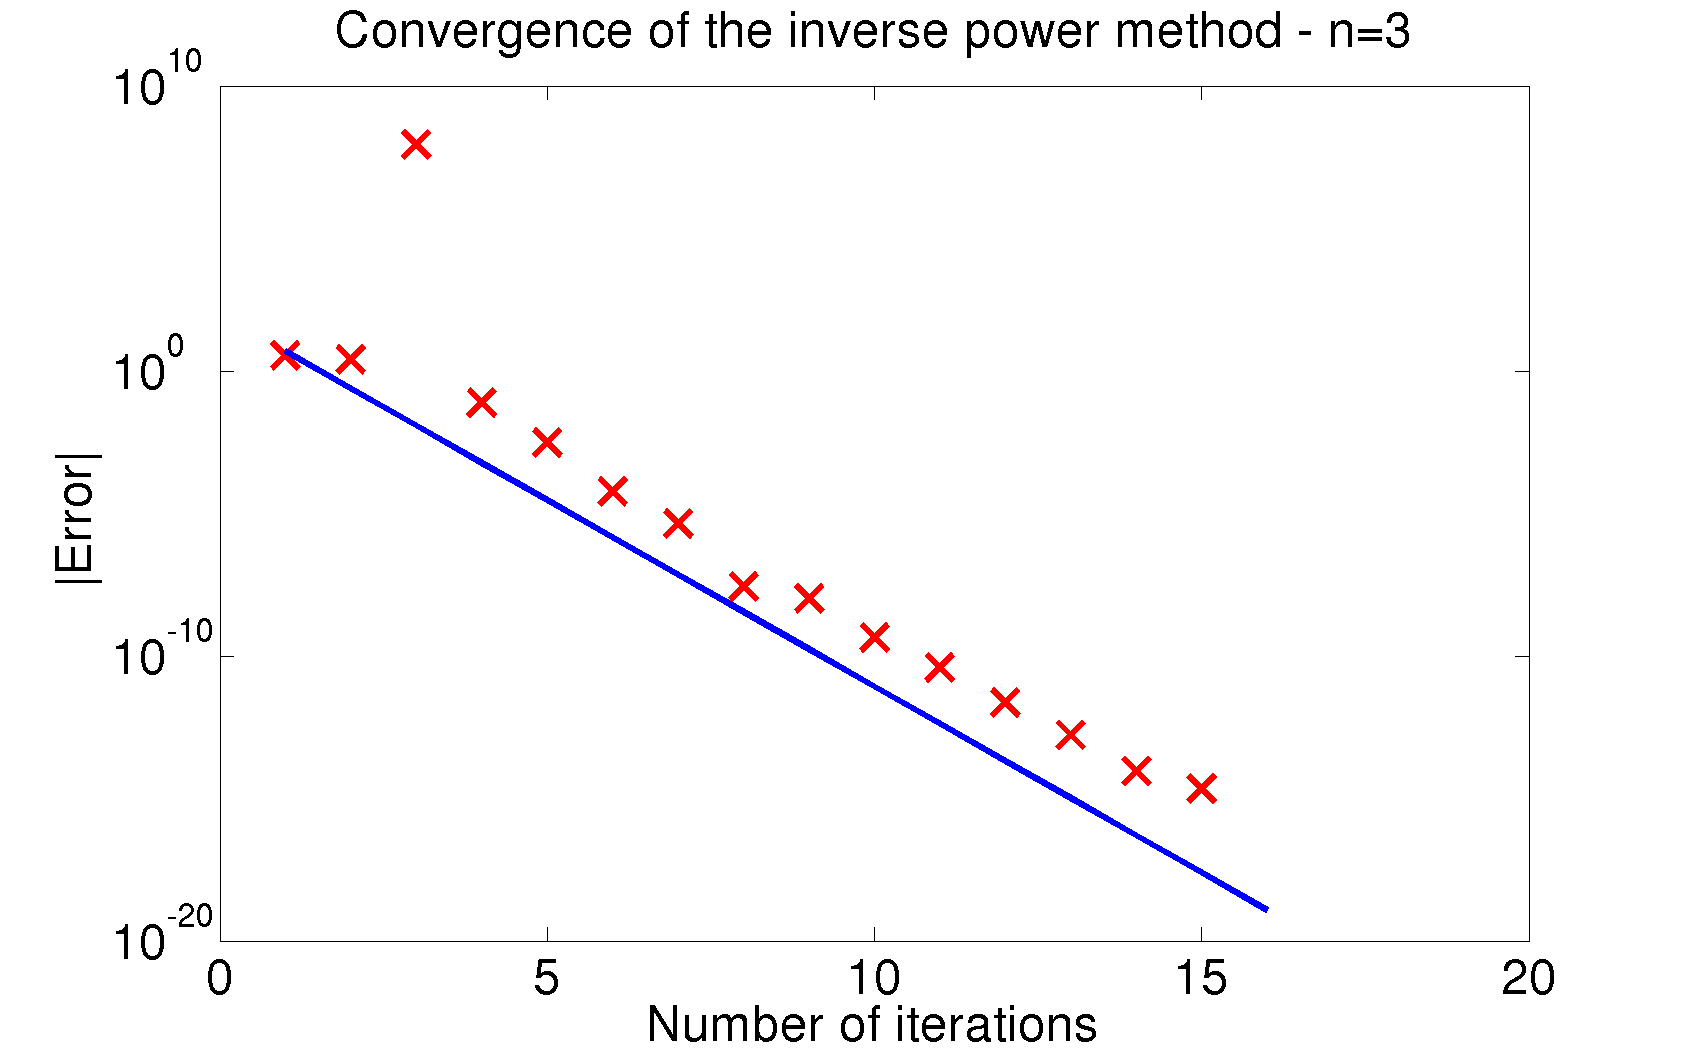
\includegraphics[width=\textwidth]{figures/InversePowerFull1}
    \end{column}
  \end{columns}

\end{frame}

\begin{frame}
  \frametitle{Shifted power method}

  Another minor variant allows us to find the eigenvalue closest to a
  given complex number $\sigma$. We just have to make use of:
  \begin{equation*}
    \lambda_i \text{ are eigenvalues of } A \Rightarrow
    \lambda_i - \sigma \text{ are eigenvalues of } A - \sigma
    \text{Id}
  \end{equation*} \pause
%
  Therefore the smallest eigenvalue of $A - \sigma \text{Id}$ is the
  one closest to $\sigma$; this is just an application of the inverse
  power method.

\end{frame}


\begin{frame}
  \frametitle{Inverse power method example}


  \begin{columns}
    \begin{column}{0.35\textwidth}
      The matrix
      \begin{equation*}
        A =
        \begin{pmatrix}
          1 & 2 & 3 \\
          4 & 5 & 6 \\
          7 & 8 & 0
        \end{pmatrix}
      \end{equation*}
      has eigenvalues
      \begin{equation*}
        \left\{
          \begin{array}{c}
            12.1229\\ -5.7345\\ -0.3884
          \end{array}\right. .
      \end{equation*}
      The shifted power method shows linear convergence to $\lambda =
      -5.7345$ for the eigenvalue closest to $-5$.
    \end{column}
    \begin{column}{0.65\textwidth}
      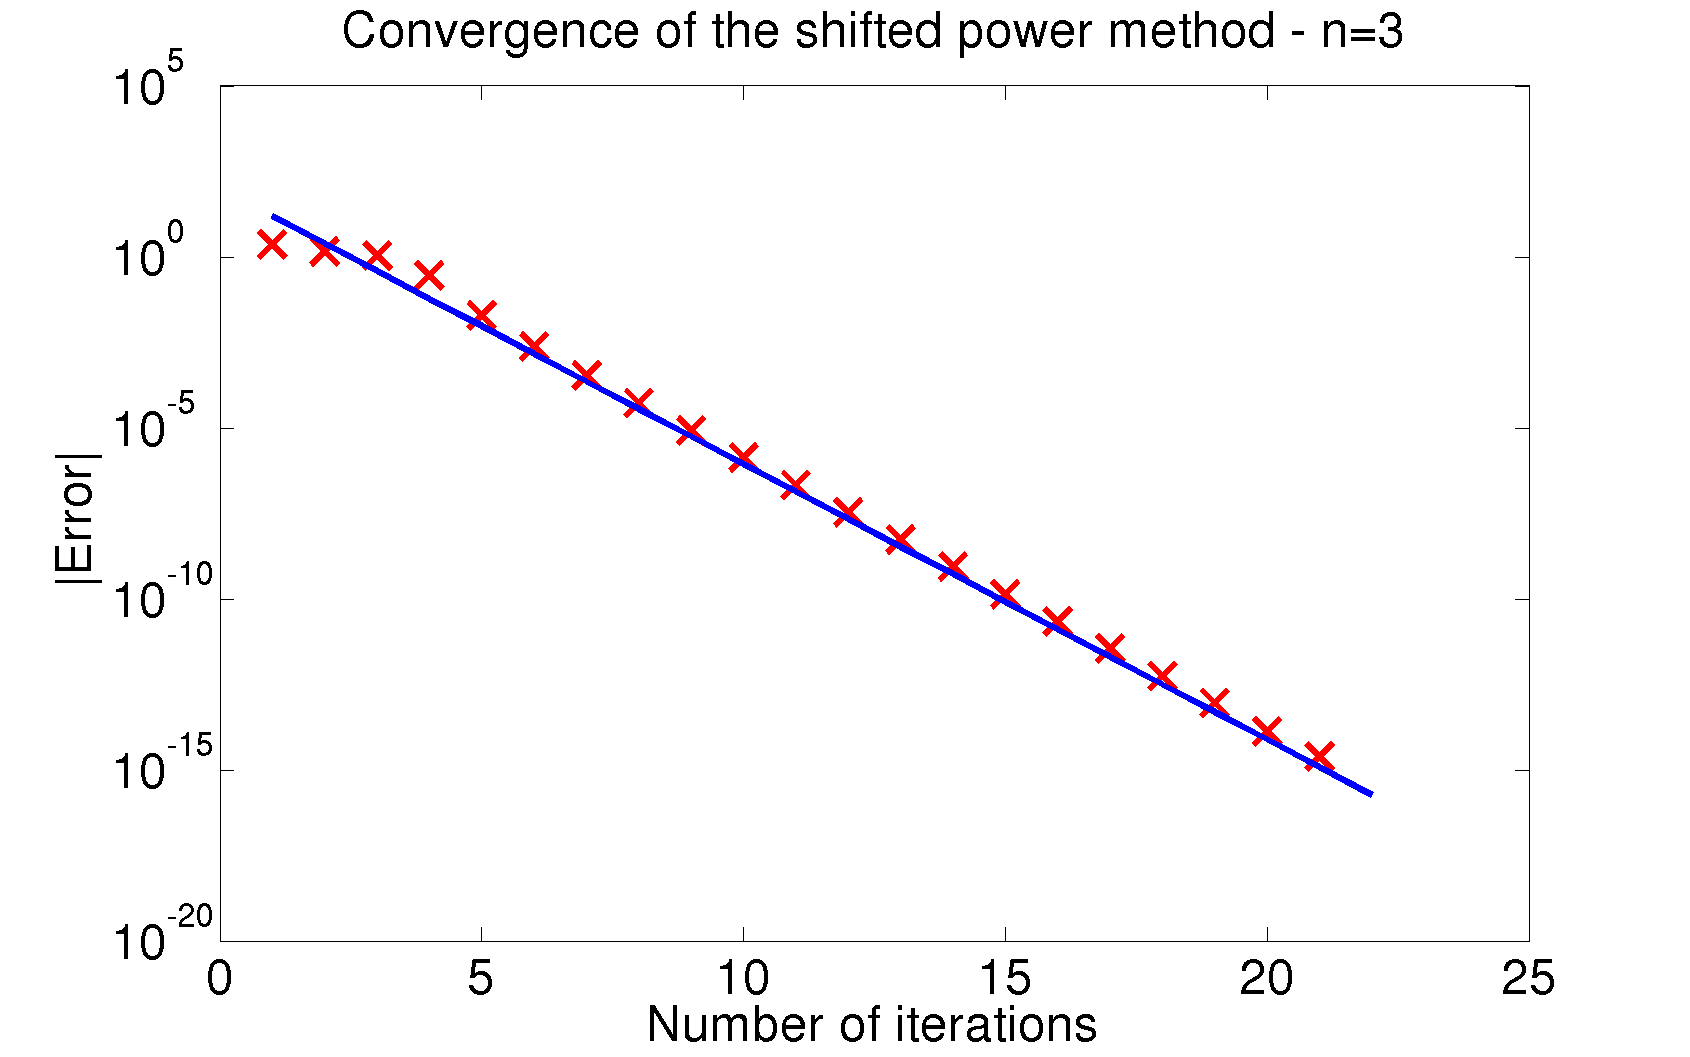
\includegraphics[width=\textwidth]{figures/ShiftedPowerFull1}
    \end{column}
  \end{columns}

\end{frame}

% \section{Informal feedback}

% \begin{frame}
%   \frametitle{Informal feedback}

%   Please write on the post-it notes
%   %
%   \begin{itemize}
%   \item \color{green}{one thing you like}
%   \item \color{red}{one thing you don't like}
%   \item \color{blue}{one thing you'd like changed \emph{this semester}}
%   \end{itemize}
%   %
%   about the module.

%   \vspace{1ex}

%   Note: only things \emph{I} can change (so not timetables, assessment weightings, etc.).

% \end{frame}

\section{The full spectrum}


\subsection{Similar matrices}

\begin{frame}
  \frametitle{Similar matrices}

  Standard trick: convert to equivalent problem that is easy to
  solve. Typical simpler problems based on diagonal or triangular
  matrices. \pause To compute \emph{all} the eigenvalues of $A$, note that
  for diagonal and triangular matrices, \emph{the eigenvalues are the
    diagonal entries}. \pause

  \vspace{1ex}

  So which matrix problems are ``equivalent''? Means the spectrum, the
  set of all eigenvalues, is unchanged. One particular useful case is
  the \emph{similarity transform}:

  {\bf Definition}: The matrices $A,B$ are similar if there exists a
  nonsingular matrix $P$ such that
  \begin{equation*}
    B = P A P^{-1}.
  \end{equation*} \pause
  %
  {\bf Theorem}: Similar matrices have the same eigenvalues.

\end{frame}

\begin{frame}
  \frametitle{Geometric interpretation of similarity transforms}

  A similarity transform expresses that the matrix equation
  \begin{equation*}
    A \bfm{u} = \bfm{v}
  \end{equation*}
  is independent of the coordinates in which it is written. \pause
  \begin{columns}
    \begin{column}{0.5\textwidth}
      Under a change of coordinates that does not move the origin, the
      vectors ``rotate'' to e.g.\
      \begin{equation*}
        \bfm{u}' = R \bfm{u}
      \end{equation*}
      for some rotation matrix $R$. \pause Hence our original equation
      becomes
      \begin{equation*}
        R A R^{-1} \bfm{u}' = \bfm{v}';
      \end{equation*}
      if the ``physical'' properties of $A$ and $R A R^{-1}$ are the
      same, then they are independent of the coordinates.
    \end{column}
    \begin{column}{0.5\textwidth}
      \begin{center}
        \includegraphics<1|handout:1>[width=\textwidth]{figures/QRRotation1}
        \includegraphics<2-|handout:2>[width=\textwidth]{figures/QRRotation2}
      \end{center}
    \end{column}
  \end{columns}

\end{frame}


\subsection{Schur's theorem}

\begin{frame}
  \frametitle{Schur's theorem}

  So we want to find a triangular matrix $B$ that $A$ is similar to;
  from that we can just read off the eigenvalues. Is this even
  possible? \pause

  \vspace{1ex}

  {\bf Schur's Theorem}: Every square matrix is unitary similar to a
  triangular matrix. \pause

  %\vspace{1ex}

  %The proof is detailed in the notes; although comforting it is
  %useless in practice as it uses the eigenvectors, which is exactly
  %the information that we are trying to find out. \pause

  \vspace{1ex}

  {\bf Corollary}: Every Hermitian matrix $A = A^{\dagger}$ is unitary
  similar to a diagonal matrix.

\end{frame}

\begin{frame}
  \frametitle{Householder reflections}

  {\bf Schur's Theorem}: Every square matrix is unitary similar to a
  triangular matrix.

  \vspace{1ex}

  One key step in the proof of the theorem is the use of
  \emph{Householder reflections}:

  \vspace{1ex}

  {\bf Lemma}: If $\bx$, $\bfm{y}$ are vectors such that $\|\bx\|_2 =
  \|\bfm{y}\|_2$ and $(\bx,\bfm{y})$ is real then the matrix $U = \text{Id} -
  \bfm{u} \bfm{u}^{\dagger}$ defined from
  \begin{equation*}
    \bfm{u} = \sqrt{2} \frac{\bx - \bfm{y}}{\|\bx - \bfm{y}\|_2}
  \end{equation*}
  gives $U \bx = \bfm{y}$. \pause

  \vspace{1ex}

  Geometric interpretation: to get $\bfm{y}$ from $\bx$,
  reflect $\bx$ in plane orthogonal to $\bfm{u}$.

\end{frame}

\begin{frame}
  \frametitle{Key steps in the proof}

  Proof of Schur's theorem by induction $n$. Obviously true
  for $n=1$ (scalar numbers). Aim: reduce matrix $A$ such that
  %
  \begin{equation*}
    U A U^{\dagger} = \left(
      \begin{array}{c|c c c}
        \mu_1 & & \bfm{w}& \\ \hline
        0 & &  & \\
        \vdots & & A_{n-1}  & \\
        0 & &  & \\
      \end{array}\right).
  \end{equation*}
  %
  I.e., rotate first column into a scalar multiple of the unit column
  vector $\hat{\bfm{e}}_1 = (1, 0, \dots 0)^T$.  \pause

  \vspace{1ex}

  Straightforward: construct appropriate Householder reflection
  %
  \begin{equation*}
    U = \text{Id} - \bfm{u}\bfm{u}^{\dagger}.
  \end{equation*}
  %
  This rotates \emph{to} $\hat{\bfm{e}}_1$; but what should it rotate
  from?

\end{frame}

\begin{frame}
  \frametitle{Key steps in the proof: 2}

  \begin{equation*}
    U A U^{\dagger} = \left(
      \begin{array}{c|c c c}
        \mu_1 & & \bfm{w}& \\ \hline
        0 & &  & \\
        \vdots & & A_{n-1}  & \\
        0 & &  & \\
      \end{array}\right).
  \end{equation*}
  %
  Want to rotate first column into scalar multiple of unit column
  vector $\hat{\bfm{e}}_1 = (1, 0, \dots 0)^T$.

  \vspace{1ex}

  Construct the appropriate Householder reflection
  \begin{equation*}
    U = \text{Id} - \bfm{u}\bfm{u}^{\dagger}.
  \end{equation*}
  This rotates \emph{to} $\hat{\bfm{e}}_1$; but what should it rotate
  from?

  \vspace{1ex}

  New matrix has $\hat{\bfm{e}}_1$ as eigenvector, eigenvalue
  $\mu_1$. Must be using an eigenvector to construct rotation;
  (suitably scaled) eigenvector is used as the vector to rotate
  \emph{from}.

\end{frame}

\begin{frame}
  \frametitle{Key steps in the proof: 3}

  The appropriate Householder reflection matrix is
  %
  \begin{align*}
    U = \text{Id} - \bfm{u}\bfm{u}^{\dagger}, & \mbox{} &
    \bfm{u} = \sqrt{2}\frac{\left( \hat{\bfm{e}}_1-\hat{\bfm{v}}_1 \right)
    }{||\hat{\bfm{e}}_1- \hat{\bfm{v}}_1||_2},
  \end{align*}
  %
  where $\hat{\bfm{v}}_1$ is the unit eigenvector with eigenvalue
  $\mu_1$.\pause

  \vspace{1ex}

  We can verify this by computing the product
  %
  \begin{align*}
    U A U^{\dagger}\hat{\bfm{e}}_1 =  \mu_1 \hat{\bfm{e}}_1
  \end{align*}
  %
  for a general square matrix and
  %
  \begin{align*}
    \hat{\bfm{e}}_1^{\dagger} U A U^{\dagger} = \mu_1 \hat{\bfm{e}}_1^{\dagger}
  \end{align*}
  %
  for an Hermitian matrix.

\end{frame}

\begin{frame}
  \frametitle{Key steps in the proof: 3}

  {\bf Schur's Theorem}: Every square matrix is unitary similar to a
  triangular matrix.

  \vspace{1ex}

  {\bf Corollary}: Every Hermitian matrix $A = A^{\dagger}$ is unitary
  similar to a diagonal matrix.

  \vspace{1ex}

  Does this help us? \pause

  \vspace{1ex}

  Although comforting, proof is useless in practice: it uses the
  eigenvectors, which is exactly the information we are trying to
  find.\pause

  \vspace{1ex}

  However, the steps used in the proof will be of fundamental importance
  in finding the full spectrum of a matrix as we will see next time.

\end{frame}
  % \subsection{\texorpdfstring{Householder's $QR$ factorisation}{Householder's QR factorisation}}



% \begin{frame}
%   \frametitle{Householder's $QR$ factorisation}

% \end{frame}

\section{Summary}

\subsection{Summary}

\begin{frame}
  \frametitle{Summary}

  \begin{itemize}
  \item The power method is an iterative procedure giving the
    eigenvalue of largest absolute modulus and its associated
    eigenvector.
  \item By looking at the inverse matrix the power method can be
    modified to give
    \begin{enumerate}
    \item the eigenvalue of smallest absolute modulus (inverse power
      method)
    \item the eigenvalue closest to a given $\sigma \in {\mathbb C}$
      (shifted inverse power method).
    \end{enumerate}
  \item To find the full spectrum it is easiest to transform the
    matrix to an ``equivalent'' diagonal or triangular matrix; in
    these cases the eigenvalues are the diagonal entries.
  \item Similar matrices $A$, $B = P A P^{-1}$ have the same
    spectrum.
  \item Schur's theorem states that every square matrix is unitary
    similar to a triangular matrix.
  \item A key step in the proof the the use of Householder
    reflections.
  \end{itemize}

\end{frame}

\end{document}



%%% Local Variables:
%%% mode: latex
%%% TeX-master: t
%%% End:
